\chapter{Аналитический раздел}\label{analysis}

\section{Анализ предметной области синхронизации игровых состояний}

\subsection{Общие положения сетевого взаимодействия}

Многопользовательские игровые приложения представляют собой распределенные системы, в которых несколько клиентов взаимодействуют с общим игровым миром через сеть~\cite{smed2002networkgames, tanenbaum2017distributed}. Для обеспечения корректности игрового процесса требуется поддерживать согласованность данных, описывающих состояние мира, действия игроков и результаты игровых событий. Сетевая передача данных сопровождается задержками, потерями пакетов, вариативностью задержки и ограничениями пропускной способности, что является одним из основных рисков возникновения рассинхронизации между участниками взаимодействия.

В отличие от одиночных игровых приложений, где состояние системы хранится и изменяется в пределах одного процесса, многопользовательское приложение должно поддерживать несколько локальных представлений одного и того же игрового мира. Каждое такое представление обновляется на основании входных действий игрока, локальной симуляции и сетевых сообщений, полученных от других участников сетевого обмена. Если порядок применения этих воздействий отличается, то даже при одинаковых исходных данных локальные состояния могут разойтись.

Наиболее распространенной архитектурой является модель с выделенным сервером, который хранит авторитетное состояние игрового мира~\cite{gamedevnetsync}. Клиенты направляют серверу информацию о своих действиях и получают обратно обновления состояния. Такая модель упрощает контроль корректности, так как сервер может проверять допустимость действий, разрешать конфликты и рассылать согласованное состояние всем участникам. В то же время серверная архитектура не устраняет сетевые задержки и не исключает временное расхождение между состоянием, отображаемым на клиенте, и состоянием, принятым сервером.

\subsection{Игровое состояние и требования к его синхронизации}

Игровое состояние представляет собой совокупность параметров, описывающих положение объектов в игровом мире, их атрибуты и поведение. К таким параметрам относятся координаты и ориентация объектов, скорость движения, состояние анимации, логические флаги, параметры здоровья, ресурсы, активные эффекты и данные о текущей фазе игрового сценария. Часть параметров изменяется непрерывно или с высокой частотой, а часть изменяется дискретно в результате игровых событий.

Для синхронизации состояний существенны два свойства:
\begin{itemize}
	\item согласованность, при которой клиентское представление состояния мира не должно существенно отличаться от авторитетного состояния;
	\item отзывчивость, при которой реакция на действия игрока должна быть визуально своевременной, несмотря на сетевые задержки.
\end{itemize}

Совместное обеспечение этих свойств представляет собой одну из основных проблем сетевых игр. Повышение отзывчивости часто достигается за счет локальной обработки ввода и временных предсказаний на клиенте. Однако такие предсказания могут не совпасть с результатом, полученным на авторитетной стороне, что приводит к необходимости корректировки состояния. В свою очередь, строгая ориентация только на подтвержденные сетевые данные уменьшает вероятность ошибки, но увеличивает задержку реакции приложения на действия пользователя.

Для игровых сценариев с непосредственным взаимодействием двух игроков особенно важны логически значимые события. В отличие от вспомогательных визуальных данных, такие события изменяют состояние системы: запускают действие, фиксируют столкновение, изменяют фазу взаимодействия, завершают ход или переводят объект в новое состояние. Потеря или повторная обработка такого события приводит не только к визуальной ошибке, но и к нарушению логики игрового процесса.

\subsection{Модели передачи данных и источники рассинхронизации}

Передача данных в многопользовательских играх может осуществляться по нескольким моделям:
\begin{itemize}
	\item снимки состояния (snapshots) --- периодическая отправка полного или частичного состояния объектов;
	\item событийная репликация (event-based sync) --- передача только событий, влияющих на состояние мира;
	\item синхронизация по входным данным (input-sync) --- передача входных команд игроков при локальном выполнении симуляции по детерминированным правилам.
\end{itemize}

Каждая модель имеет свои ограничения. Передача снимков состояния упрощает восстановление клиентского представления, но требует значительного объема трафика при большом количестве объектов. Событийная репликация экономит сетевые ресурсы, но зависит от корректной и одинаковой обработки событий на всех сторонах взаимодействия. Синхронизация по входным данным обеспечивает низкое сетевое потребление, однако предъявляет высокие требования к детерминизму симуляции и одинаковости вычислений на всех клиентах.

Основные источники рассинхронизации включают:
\begin{itemize}
	\item сетевые задержки и их вариативность;
	\item потерю, дублирование и нарушение порядка доставки пакетов;
	\item недетерминированность клиентской симуляции;
	\item различия в частоте обновления и производительности устройств;
	\item асинхронность обработки событий.
\end{itemize}

Для рассматриваемой работы наибольшее значение имеет рассинхронизация, возникающая из-за неодинакового порядка обработки событий. Если одно событие переводит систему из состояния $q_i$ в состояние $q_j$, то применение другого события до завершения этого перехода может оказаться недопустимым. Следовательно, синхронизация должна включать не только передачу сообщения, но и проверку того, что событие применимо к текущему состоянию системы.

\subsection{Факторы, влияющие на требования к синхронизации}

Требования к точности и частоте синхронизации существенно отличаются в зависимости от жанра игры:
\begin{itemize}
	\item FPS и экшен-игры требуют высокой частоты обновления и минимальной задержки, поскольку ошибки в позиции или времени приводят к критичным изменениям игрового процесса;
	\item MOBA и RPG допускают более низкую частоту синхронизации, поскольку взаимодействия менее чувствительны к малым задержкам;
	\item RTS часто используют детерминированную модель мира и обмен только входными данными для повышения масштабируемости.
\end{itemize}

Помимо жанра, важными факторами являются количество игроков и объектов в сцене, нагрузка на сеть, ограничения пропускной способности, необходимость поддержки слабых клиентских устройств и плотность взаимодействия игроков друг с другом. Чем выше плотность взаимодействия, тем больше вероятность конфликтов между событиями и тем строже должны быть правила их обработки.

В случае двух игроков требования к пропускной способности ниже, чем в массовых многопользовательских системах, однако требования к корректности обработки событий остаются высокими.

\section{Формализация задачи обеспечения согласованности игровых данных}

\subsection{Математическое представление игрового состояния}

Игровой мир многопользовательского приложения можно представить в виде динамической системы, состояние которой изменяется во времени под воздействием действий игроков и игровой логики. Состояние мира в момент времени $t$ обозначим как $S(t)$:
\[
	S(t) = \{ s_1(t), s_2(t), \ldots, s_n(t) \},
\]
где $s_i(t)$ --- состояние $i$-й игровой сущности.

Каждое состояние можно формально представить как вектор параметров:
\[
	s_i(t) = \left( p_i(t), v_i(t), a_i(t), \lambda_i(t) \right),
\]
где:
\begin{itemize}
	\item $p_i(t)$ --- позиция сущности;
	\item $v_i(t)$ --- скорость;
	\item $a_i(t)$ --- параметры активности или выполняемого действия;
	\item $\lambda_i(t)$ --- дискретные состояния и флаги.
\end{itemize}

Все состояние мира представляет собой многомерное пространство, которое необходимо корректно поддерживать на взаимодействующих сторонах. Для двух игроков состояние можно представить как объединение локальных состояний игроков и состояния общих объектов:
\[
	S(t) = \left(S_1(t), S_2(t), S_c(t)\right),
\]
где:
\begin{itemize}
	\item $S_1(t)$ --- состояние первого игрока;
	\item $S_2(t)$ --- состояние второго игрока;
	\item $S_c(t)$ --- состояние общих сущностей и параметров взаимодействия.
\end{itemize}

В событийной модели изменение состояния вызывается событием $e \in E$, где $E$ --- множество допустимых игровых событий. Тогда переход состояния можно описать функцией:
\[
	S(t + \Delta t) = F(S(t), e),
\]
где $F$ --- функция применения события к текущему состоянию.

\subsection{Модель клиент-серверного взаимодействия}

В большинстве сетевых игр сервер является источником авторитетного состояния. Клиентская сторона может оперировать временными предсказаниями, но окончательные значения состояния принадлежат серверу. На стороне клиента поддерживается приближенное состояние $\hat{S}(t)$, которое может отличаться от серверного $S(t)$.

Клиент получает обновления состояния в дискретные моменты времени $t_k$:
\[
	S(t_k) \rightarrow \text{клиент},
\]
а отправляет данные о действиях игрока в форме входных команд:
\[
	u(t_k) = \text{input}(t_k), \qquad u(t) \in U,
\]
где $U$ --- пространство возможных действий.

Сервер выполняет симуляцию:
\[
	S(t + \Delta t) = F(S(t), u_1(t), u_2(t), \ldots, u_m(t)),
\]
где $F$ --- функция игровой логики, $m$ --- количество игроков.

Для событийной синхронизации входная команда может рассматриваться как причина формирования события. В этом случае сетевое взаимодействие описывается передачей сообщения $m_k$, содержащего событие $e_k$, его идентификатор, номер последовательности и служебные параметры доставки. Если сообщение потеряно или обработано не в том порядке, то соответствующее событие может быть применено некорректно или не применено вовсе.

\subsection{Определение рассогласования состояния}

Пусть клиентское состояние $\hat{S}(t)$ является приближением авторитетного состояния $S(t)$. Тогда показатель рассогласования можно определить следующим образом:
\[
	D(S(t), \hat{S}(t)) = \sum_{i=1}^{n} w_i \cdot d(s_i(t), \hat{s}_i(t)),
\]
где $d()$ --- расстояние между состояниями одной сущности, $w_i$ --- вес значимости сущности.

Функция $d()$ может включать позиционную ошибку, ошибку скорости и различие дискретных параметров:
\[
	d(s_i, \hat{s}_i) =
	\alpha \cdot \|p_i - \hat{p}_i\| +
	\beta \cdot \|v_i - \hat{v}_i\| +
	\gamma \cdot \delta(\lambda_i, \hat{\lambda}_i),
\]
где:
\begin{itemize}
	\item $\|p_i - \hat{p}_i\|$ --- расстояние между фактической позицией сущности и ее клиентским приближением;
	\item $\|v_i - \hat{v}_i\|$ --- разница скоростей сущности;
	\item $\delta(\lambda_i, \hat{\lambda}_i)$ --- бинарная функция различия дискретных параметров;
	\item $\alpha$, $\beta$, $\gamma$ --- веса значимости соответствующих ошибок.
\end{itemize}

Бинарная функция различия дискретных параметров задается следующим образом:
\[
	\delta(\lambda_i, \hat{\lambda}_i) =
	\begin{cases}
		0, & \text{если } \lambda_i = \hat{\lambda}_i,\\
		1, & \text{если } \lambda_i \neq \hat{\lambda}_i.
	\end{cases}
\]

Допустимый порог рассогласования определим как:
\[
	D(S(t), \hat{S}(t)) \leqslant D_{\text{max}}.
\]
Если ошибка превышает порог, требуется корректировка состояния или повторная обработка событий, приведших к расхождению.

Для дискретной событийной логики существенна не только численная ошибка параметров, но и совпадение логических состояний. Если два игрока имеют одинаковые координаты объектов, но находятся в разных состояниях конечного автомата взаимодействия, например один клиент считает действие завершенным, а другой --- выполняющимся, система остается несогласованной. Поэтому при разработке метода необходимо учитывать как параметрическое, так и логическое рассогласование.

\subsection{Постановка задачи обеспечения согласованности}

Целью системы синхронизации является минимизация рассогласования между локальными представлениями состояния при ограничениях на сетевые ресурсы и задержки:
\[
	\min_{\Pi} \; D\left(S(t), \hat{S}_{\Pi}(t)\right),
\]
где $\Pi$ --- выбранный алгоритм синхронизации.

При этом должны выполняться следующие ограничения:
\[
	B(\Pi) \leqslant B_{\text{max}}, \qquad
	L(\Pi) \leqslant L_{\text{max}},
\]
где:
\begin{itemize}
	\item $B(\Pi)$ --- требуемая пропускная способность;
	\item $L(\Pi)$ --- задержка реакции;
	\item $B_{\text{max}}$ --- допустимое ограничение пропускной способности сети;
	\item $L_{\text{max}}$ --- допустимое ограничение задержки реакции.
\end{itemize}

В общем виде задача синхронизации представляет собой многокритериальную оптимизацию:
\[
	\min_{\Pi} \left(
		\alpha \cdot D +
		\beta \cdot B +
		\gamma \cdot L
	\right),
\]
где:
\begin{itemize}
	\item $\alpha$ --- вес важности согласованности;
	\item $\beta$ --- вес важности трафика;
	\item $\gamma$ --- вес важности задержки.
\end{itemize}

Для разрабатываемого метода важно, что минимизация рассогласования должна достигаться не только за счет более частой передачи данных. Увеличение частоты сообщений повышает нагрузку на сеть и не устраняет проблему нарушения порядка событий. Поэтому требуется метод, который ограничивает множество допустимых переходов состояния и обеспечивает корректную обработку событий даже при ненадежной доставке сообщений.

Формализованная постановка задачи представлена в виде IDEF0-диаграммы на рисунке~\ref{img:analysis-idef0-task}.

\begin{figure}[H]
	\centering
	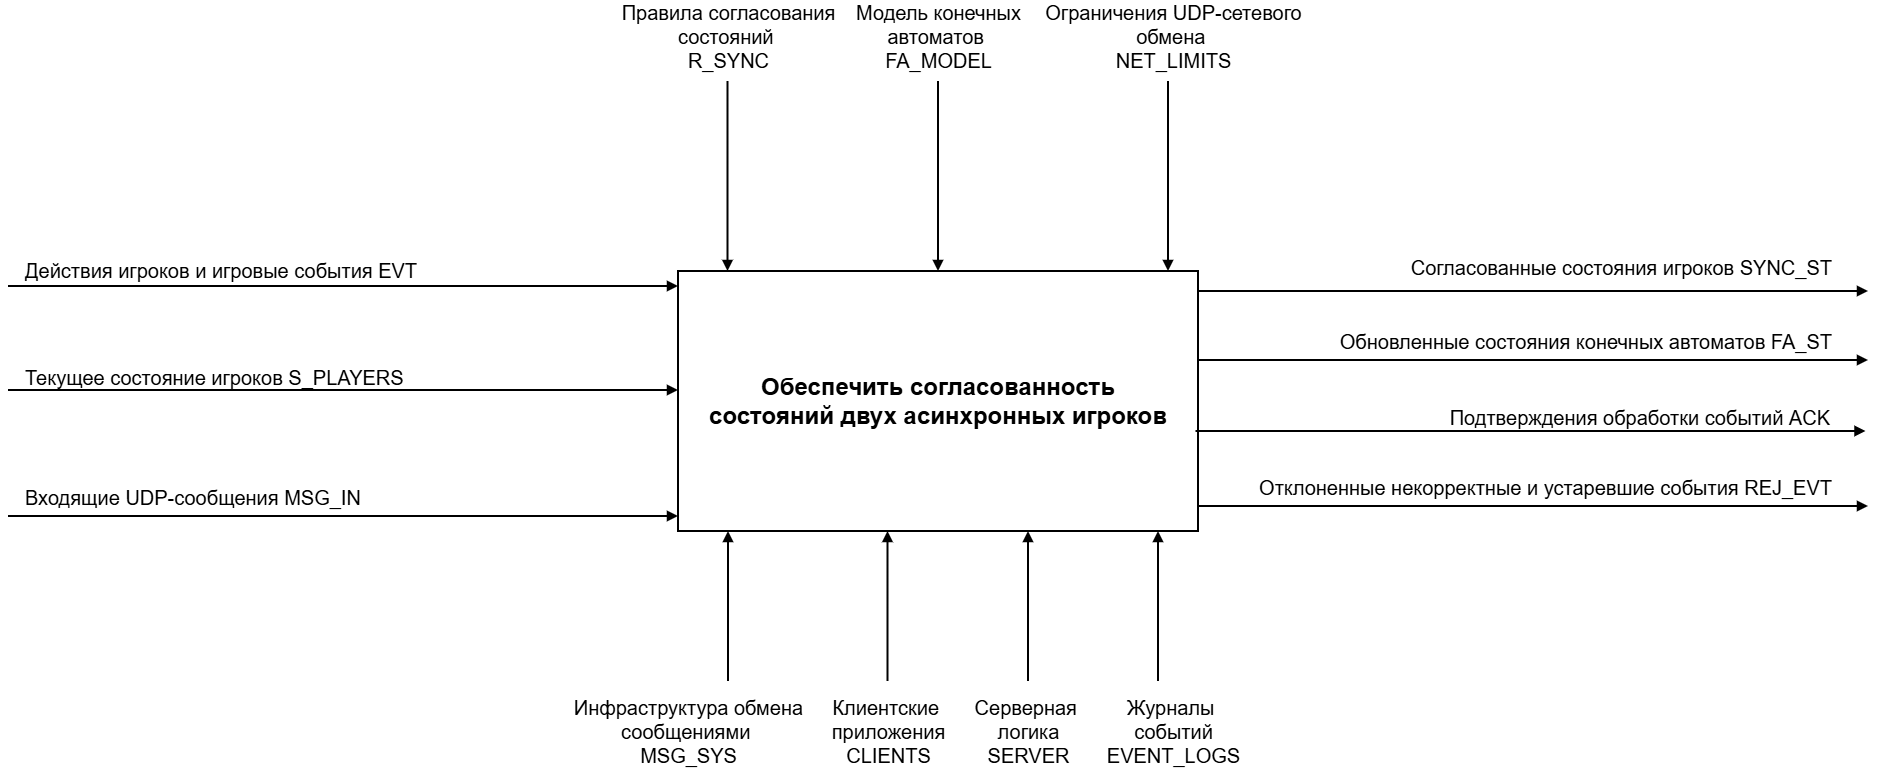
\includegraphics[width=\textwidth]{inc/img/idef0.png}
	\caption{IDEF0-диаграмма постановки задачи обеспечения согласованности состояний}
	\label{img:analysis-idef0-task}
\end{figure}

\subsection{Требования к алгоритмам синхронизации}

Алгоритмы, обеспечивающие согласованность игровых состояний, должны удовлетворять следующим требованиям:
\begin{itemize}
	\item точность --- алгоритм должен обеспечивать минимальные расхождения между состояниями, чтобы игроки наблюдали корректную картину происходящего;
	\item стабильность --- изменения состояния и корректировки должны происходить без резких скачков и визуальных искажений;
	\item устойчивость к сетевым ошибкам --- система должна корректно работать при задержках, потере отдельных пакетов, дублировании и нарушении порядка доставки;
	\item эффективность --- алгоритм не должен перегружать вычислительные ресурсы и должен использовать ограниченный объем сетевого трафика;
	\item проверяемость переходов --- система должна иметь возможность определить, допустимо ли входное событие в текущем состоянии;
	\item воспроизводимость обработки --- одинаковая последовательность событий должна приводить к одинаковому результату на всех участниках взаимодействия.
\end{itemize}

Задача обеспечения согласованности игровых данных формализуется как задача управления состоянием распределенной асинхронной системы, в которой необходимо уравновесить точность, задержку реакции, сетевую нагрузку и корректность обработки событий.

\section{Обзор существующих подходов к синхронизации состояния}

Механизмы синхронизации состояния определяют, каким образом сервер и клиенты обеспечивают актуальность игрового мира, минимизируя расхождения между расчетами на стороне сервера и восприятием игрока. Ниже рассмотрены основные методы, используемые в современных сетевых играх различных жанров.

\subsection{Периодическая репликация состояния}

При использовании снимков сервер с фиксированной частотой отправляет клиентам актуальное состояние мира или его части~\cite{valvesource}. Снимок включает координаты и характеристики активных объектов, состояние игровых сущностей и флаги игровой логики. Этот подход используется в шутерах и других динамичных играх, где важна высокая частота обновления положения объектов и событий~\cite{unity_netcode_docs}.

Преимуществами периодической репликации состояния являются простота реализации и высокая точность согласования при стабильной сети. Клиент регулярно получает авторитетные данные и может восстанавливать свое представление мира даже после потери отдельного обновления.

Недостатками подхода являются высокий объем трафика при большом числе объектов, возможные скачки состояния при применении обновлений и чувствительность к потере последовательных пакетов. Кроме того, передача снимков состояния не описывает причин перехода из одного состояния в другое. Поэтому данный подход хуже подходит для анализа логически значимых событий, которые должны быть применены строго один раз и в определенном порядке.

\subsection{Репликация только изменений}

При репликации изменений сервер отправляет не полный снимок, а только параметры, которые изменились со времени последнего известного клиенту состояния~\cite{unreal_replicate}. Данный метод применяется в системах, где полный снимок мира передавать нецелесообразно из-за большого количества объектов.

Преимуществами метода являются снижение объема передаваемых данных и эффективная работа в больших сценах. Если изменения затрагивают небольшую часть объектов, передача только измененных параметров существенно уменьшает сетевую нагрузку.

К недостаткам относится необходимость хранить предыдущее состояние, относительно которого вычисляется изменение. При потере сообщения клиент может оказаться в состоянии, к которому последующая дельта неприменима. В результате возможно накопление ошибок, поэтому такие системы обычно нуждаются в периодической отправке полного состояния для восстановления согласованности.

\subsection{Событийная модель}

В рамках событийной модели участникам передаются сведения не о полном состоянии объектов, а о произошедших событиях~\cite{GameEventSync2008}. Событие описывает действие, которое должно быть применено к текущему состоянию: начало движения, взаимодействие с объектом, изменение режима, столкновение, создание или уничтожение сущности.

Событийная модель часто используется в RPG, MOBA и стратегиях, где значительная часть взаимодействий описывается дискретными событиями. Преимуществами подхода являются малый объем передаваемых данных, высокая эффективность для логических действий и совместимость с детерминированной симуляцией.

Главная сложность событийной модели заключается в необходимости одинаковой обработки событий на всех сторонах взаимодействия. Если событие потеряно, обработано повторно или применено в неправильном состоянии, локальные представления мира расходятся. Поэтому для событийной синхронизации особенно важны контроль порядка, идентификаторы событий, подтверждения доставки и проверка допустимости переходов.

Данный подход является наиболее близким к теме работы, так как конечный автомат может быть использован для формального описания того, какие события допустимы в каждом состоянии и к каким переходам они приводят.

\subsection{Синхронизация по входным данным}

При синхронизации по входным данным сервер или другой координирующий компонент рассылает клиентам не состояние, а входные команды игроков. Детерминированная симуляция на всех системах должна приводить к одинаковому результату~\cite{photon_sync}.

Этот подход характерен для стратегий в реальном времени, файтингов и симуляторов, где критично поддерживать строгий детерминизм. Преимуществами являются минимальное сетевое потребление и высокая согласованность при условии, что симуляция действительно детерминирована.

Недостатки связаны со сложностью обеспечения детерминизма. Разные процессоры, разные реализации операций с плавающей точкой, отличия в частоте кадров и порядок обновления объектов могут привести к несовпадению результатов. Кроме того, необходимо синхронизировать тики симуляции и очереди входных команд, что повышает сложность реализации.

\subsection{Предсказание состояния на клиенте}

При клиентском предсказании клиент применяет действие игрока немедленно после ввода, не ожидая ответа сервера~\cite{claypool2010latency}. После получения авторитетных данных выполняется проверка и, при необходимости, корректировка состояния.

Механизм предсказания широко используется в динамичных шутерах и экшен-играх, требующих минимальной задержки отклика на ввод игрока. Преимуществами являются высокая отзывчивость управления и снижение субъективного влияния сетевой задержки.

Недостатками являются возможные рывки при корректировке, риск накопления ошибок при нестабильной сети и усложнение логики восстановления состояния. Для логически значимых событий предсказание особенно рискованно, так как ошибка может затронуть не только координаты объекта, но и состояние всей системы взаимодействия.

\subsection{Откат сетевого кода}

Метод отката используется в играх с высокой чувствительностью к синхронизации действий. Клиент предсказывает действия другого участника, а после получения реальных данных выполняется откат состояния и повторный расчет симуляции~\cite{ggpo}. Rollback-подход применяется в аркадных PvP-играх и проектах с высокой чувствительностью к точности столкновений.

Преимуществами метода являются высокая точность взаимодействий и уменьшение видимого влияния сетевой задержки. Недостатками являются повышенная нагрузка на вычислительные ресурсы, необходимость хранить историю состояний и возможные визуальные искажения при пересчете.

Для разрабатываемого метода rollback-подход важен как пример обработки сетевой асинхронности через историю состояний. Однако в рассматриваемой задаче основной акцент делается не на пересчете физической симуляции, а на управлении допустимыми переходами дискретных состояний с помощью конечного автомата.

\section{Обзор методов передачи игровых данных}

\subsection{Надежная и ненадежная доставка данных}

В сетевых играх используются два основных подхода к передаче пакетов: надежная доставка и доставка без гарантий получения~\cite{kurose2013networking}. Они различаются по задержке, стабильности и объему служебной информации.

Надежная доставка, основанная на протоколе TCP, обеспечивает контроль целостности данных и сохраняет порядок передачи пакетов, повторно отправляя утраченные сегменты~\cite{stevens2011tcpip}. Такая модель удобна для передачи данных, потеря которых недопустима. Однако TCP добавляет задержку из-за механизма подтверждений, повторных передач и сохранения общего порядка байтового потока. Для динамичных игр с высокой частотой обновления состояния это может приводить к задержке обработки новых данных из-за ожидания восстановления старых сегментов.

Ненадежная доставка, реализованная через протокол UDP, не гарантирует получение каждого отдельного пакета, но обеспечивает меньшие накладные расходы и минимально возможную задержку. Большинство сетевых игр используют UDP и собственные механизмы надежности для критичных данных. Такой подход позволяет выбирать, какие сообщения требуют подтверждения и повторной отправки, а какие могут быть потеряны без нарушения логики.

Для разрабатываемого метода использование UDP означает, что контроль доставки, порядка и дублирования логически значимых событий должен выполняться на прикладном уровне. Это соответствует событийной природе метода: не все данные требуют надежной передачи, но события, приводящие к переходам конечного автомата, должны быть обработаны согласованно.

\subsection{Классификация и приоритизация игровых пакетов}

Игровые данные по-разному реагируют на задержки и потери, поэтому пакеты обычно разделяют на классы приоритетности. Это позволяет оптимизировать передачу и избежать перегрузки канала связи.

Критичные данные включают команды игрока, результаты столкновений и важные события игровой логики. Они должны доставляться максимально быстро и целостно, поскольку их потеря может привести к заметной рассинхронизации состояния.

Важные, но допускающие потерю данные могут передаваться чаще, но без гарантии получения. Потеря части таких пакетов компенсируется новыми обновлениями в следующих сообщениях. Примером являются часто обновляемые координаты объектов, когда более новое значение делает устаревшее сообщение неактуальным.

Второстепенные данные, например визуальные эффекты, косметические параметры и отдельные звуковые события, могут передаваться с низким приоритетом или не передаваться вовсе, если клиент способен корректно воспроизводить их локально.

В контексте данной работы к критичным данным относятся события, изменяющие состояние конечного автомата. Такие события должны иметь идентификатор, номер последовательности и признак подтверждения, чтобы принимающая сторона могла обнаружить потерю, повтор или нарушение порядка.

\subsection{Механизмы обеспечения частичной надежности}

Поскольку UDP сам по себе не предоставляет гарантированную доставку, игровые движки внедряют дополнительные механизмы частичной надежности, позволяющие гарантировать передачу важных данных без превращения всего обмена в аналог TCP.

К таким механизмам относятся:
\begin{itemize}
	\item подтверждение доставки для отдельных типов пакетов;
	\item повторная отправка важных данных при отсутствии подтверждения;
	\item нумерация пакетов для восстановления порядка исполнения команд;
	\item фильтрация дубликатов по идентификаторам сообщений;
	\item отбрасывание устаревших сообщений, которые относятся к уже пройденному состоянию системы.
\end{itemize}

Эти механизмы позволяют экономно расходовать сетевой ресурс, сохраняя критичные данные в актуальном состоянии. При этом важно, чтобы повторная отправка не приводила к повторному применению одного и того же события. Поэтому прикладный уровень должен различать доставку сообщения и применение события к состоянию системы.

\subsection{Адаптивные алгоритмы передачи данных}

Современные сетевые игры используют динамические методы, которые подстраиваются под качество канала. Адаптивные алгоритмы позволяют снижать нагрузку в условиях высокой задержки или потери пакетов и увеличивать точность передачи при стабильном соединении.

К распространенным техникам относятся:
\begin{itemize}
	\item изменение частоты отправки пакетов в зависимости от текущей задержки;
	\item снижение точности квантования при перегрузке сети;
	\item динамическое отключение второстепенных данных;
	\item регулирование частоты отправки обновлений в зависимости от важности объектов.
\end{itemize}

Такие методы повышают устойчивость сетевой игры при различных условиях соединения и снижают риск возникновения рассинхронизации. Однако они не заменяют механизмы согласования событий. Если логически значимое событие потеряно или обработано в неверном состоянии, уменьшение частоты передачи второстепенных данных не восстановит корректность системы.

\section{Типовые игровые данные, подлежащие хранению, обновлению и передаче}

В процессе работы многопользовательского игрового приложения сервер и клиенты обмениваются различными типами данных, описывающих состояние объектов, игровые события и вспомогательные параметры~\cite{gregory2018gamedev}. Эти данные определяют внутреннюю логику игрового мира и корректность взаимодействия игроков.

\subsection{Данные состояния объектов}

Состояние объектов описывает характеристики сущностей и является основой игрового мира. Эти данные подлежат частому обновлению.

К типичным данным состояния объектов относятся:
\begin{itemize}
	\item позиция объекта;
	\item скорость и направление движения;
	\item поворот и ориентация;
	\item состояние анимации;
	\item физические параметры.
\end{itemize}

Эти данные требуют высокой точности и частой синхронизации. Особенно это критично для FPS, гонок и экшен-игр, где любое отклонение в позиции приводит к заметным ошибкам восприятия. В то же время часть таких данных может устаревать: если новое значение позиции уже получено, старое значение обычно не требуется применять.

\subsection{Данные игровой логики}

Помимо визуального состояния объектов существуют параметры, влияющие на игровую логику.

В эту категорию входят:
\begin{itemize}
	\item здоровье;
	\item ресурсы;
	\item активные эффекты;
	\item флаги состояний;
	\item текущая фаза взаимодействия.
\end{itemize}

Данные игровой логики обновляются реже, чем параметры движения, но требуют более надежной доставки. Ошибка в таких данных приводит к различию в результатах игровых событий. Например, если один участник считает, что действие уже завершено, а другой продолжает считать его активным, то последующие события будут интерпретированы по-разному.

\subsection{Данные взаимодействия и событий}

Игровые события отображают дискретные изменения состояния мира. Они могут быть результатом действий игрока или следствием внутренних механик.

Примеры событий:
\begin{itemize}
	\item совершение действия;
	\item взаимодействие с объектом;
	\item создание или уничтожение объекта;
	\item начало или завершение игровой фазы;
	\item срабатывание триггера.
\end{itemize}

События требуют надежной обработки, поскольку их потеря приводит к расхождениям в симуляции между игроками. Кроме того, событие должно применяться в определенном состоянии системы. Если событие доставлено позже, чем система перешла в следующее состояние, оно может стать устаревшим и должно быть обработано особым образом.

Именно данные взаимодействия и событий являются основным объектом рассмотрения в разрабатываемом методе. Для них необходимо обеспечить доставку, порядок, защиту от повторного применения и проверку допустимости перехода.

\subsection{Вспомогательные данные}

Некоторые игры используют дополнительные данные, не относящиеся напрямую к состоянию объектов, но влияющие на корректность симуляции.

К таким данным относятся:
\begin{itemize}
	\item навигационные сетки;
	\item вспомогательные маркеры;
	\item данные о временных параметрах;
	\item параметры конфигурации игровой сессии.
\end{itemize}

Эти данные чаще хранятся на сервере и передаются клиенту при необходимости. Их изменение обычно происходит реже, чем изменение состояния объектов, однако несогласованность таких данных может привести к разному поведению симуляции на разных сторонах.

\subsection{Визуальные данные}

Некоторые данные не влияют на игровую логику напрямую и могут синхронизироваться реже или генерироваться на клиенте без участия сервера.

К таким данным относятся:
\begin{itemize}
	\item эффекты частиц;
	\item косметические параметры;
	\item звуковые события;
	\item вспомогательные элементы интерфейса.
\end{itemize}

Передача таких данных оптимизируется в первую очередь при ограничении пропускной способности. Потеря визуального события может ухудшить восприятие, но обычно не приводит к нарушению логики взаимодействия.

\subsection{Метаданные и технические данные}

Помимо игровых данных существует набор технической информации, обеспечивающей корректную работу сетевого взаимодействия.

К ним относятся:
\begin{itemize}
	\item идентификаторы объектов;
	\item временные метки;
	\item номера последовательности;
	\item контрольные суммы;
	\item служебные флаги;
	\item идентификаторы подтверждений доставки.
\end{itemize}

Такие данные не видны игроку, но они важны для поддержания согласованности состояния и предотвращения ошибок. В методе, основанном на конечных автоматах, технические данные используются для связи сетевого сообщения с конкретным событием, состоянием автомата и фактом обработки этого события.

\section{Основные причины возникновения рассинхронизации}

Рассинхронизация состояния --- это расхождение между данными, хранящимися на авторитетной стороне, и состоянием, которое отображается или обрабатывается в клиентских приложениях. Возникновение рассинхронизации обусловлено как особенностями сетевого окружения, так и архитектурными проблемами внутри игрового приложения.

\subsection{Сетевые задержки}

Одной из наиболее распространенных причин рассинхронизации является задержка передачи данных~\cite{pantel2002lag}. Игровой клиент всегда получает состояние с определенной задержкой, зависящей от качества соединения. Если задержка непостоянна и резко меняется, клиент может получить обновления позже или раньше ожидаемого момента, что вызывает временные расхождения в позициях объектов и фазах событий.

Ситуация ухудшается в условиях нестабильных сетей, где вариативность задержек возрастает. Для событийной синхронизации это означает, что событие, созданное раньше, может быть доставлено позже события, созданного после него. Без контроля порядка такая ситуация приводит к некорректной последовательности переходов состояния.

\subsection{Потеря, дублирование и нарушение порядка доставки пакетов}

При использовании ненадежных протоколов часть пакетов может теряться или приходить в другом порядке. Это приводит к следующим ошибкам:
\begin{itemize}
	\item объект остается на устаревшей позиции;
	\item проигрываются неактуальные события;
	\item происходит откат состояния назад;
	\item одно и то же событие применяется несколько раз;
	\item переход состояния выполняется без необходимого предшествующего события.
\end{itemize}

Хотя игровые движки реализуют механизмы частичной надежности, абсолютной защиты от подобных проблем нет. Поэтому прикладная логика должна быть готова к получению некорректных, повторных и устаревших сообщений.

\subsection{Недетерминизм симуляции}

Некоторые игры опираются на локальный расчет физики или игровой логики на стороне клиента. Любое незначительное отличие в вычислениях может привести к расхождению состояния. Основные источники недетерминизма:
\begin{itemize}
	\item использование чисел с плавающей точкой, дающих разные результаты на разных процессорах;
	\item различный порядок обновления объектов на разных клиентах;
	\item вариации частоты кадров, влияющие на расчет физики.
\end{itemize}

Такие проблемы особенно заметны в стратегиях и симуляторах, где большое количество объектов должно развиваться по одинаковым правилам в течение длительного времени. В задачах с конечными автоматами недетерминизм проявляется как неодинаковое выполнение переходов при одинаковых входных событиях, что делает систему непредсказуемой.

\subsection{Различия в производительности клиентских устройств}

Игровые клиенты могут работать с разной скоростью в зависимости от мощности процессора, видеокарты и текущей нагрузки. Если частота обновления симуляции отличается, одни клиенты рассчитывают больше физических шагов, чем другие, а предсказания состояния расходятся с авторитетной логикой.

В играх, где симуляция сильно зависит от стабильной частоты кадров, такие различия являются источником ошибок. Для снижения влияния этого фактора часто используется фиксированный шаг симуляции, синхронизация тиков и отделение логического состояния от частоты отрисовки.

\subsection{Неправильная или неполная сериализация данных}

При передаче состояния объекты сериализуются. Ошибки сериализации приводят к тому, что данные не совпадают на клиенте и сервере. Это может быть вызвано:
\begin{itemize}
	\item пропуском некоторых параметров объекта;
	\item отправкой данных в неправильном формате;
	\item несогласованностью типов при чтении и записи;
	\item различием версий протокола обмена.
\end{itemize}

Для событийной модели ошибка сериализации особенно опасна, если затрагивает идентификатор события, номер последовательности, тип события или состояние, к которому оно относится. В этом случае сообщение может быть доставлено, но обработано как другое событие или как событие для другого состояния.

\subsection{Несогласованный порядок выполнения событий}

Если события обрабатываются не в том же порядке, что на авторитетной стороне, результаты симуляции расходятся. Это происходит из-за локальных оптимизаций клиента, попадания пакетов с разными временными метками, параллельного выполнения задач и применения предсказания до получения подтверждения от сервера.

Несогласованная обработка событий особенно критична для игр с динамичными механиками взаимодействия. Например, если событие завершения действия обработано раньше события его начала, система может перейти в недопустимое состояние. Поэтому порядок событий должен контролироваться не только на транспортном уровне, но и на уровне модели состояний.

\subsection{Ошибки в предсказании и последующей коррекции состояния}

Клиентское предсказание значительно повышает отзывчивость, но несет риск ошибок. Предсказание может расходиться с реальными данными сервера, что приводит к резким скачкам при корректировке, неверным расчетам следующего состояния и накоплению ошибки при плохой связи~\cite{gamenetpatterns}.

Такие проблемы заметны при нестабильной задержке сети и большом количестве корректировок. В дискретной логике взаимодействия ошибка предсказания может привести к тому, что клиент временно перейдет в состояние, которое затем будет отклонено авторитетной стороной. В этом случае система должна иметь способ безопасно отменить или скорректировать переход.

\section*{Вывод}

В данном разделе была рассмотрена предметная область синхронизации игровых состояний в многопользовательских приложениях. 
Было показано, что такие приложения являются распределенными асинхронными системами, в которых рассинхронизация может возникать из-за задержек, потерь пакетов, нарушения порядка доставки, 
недетерминизма симуляции и неодинаковой обработки событий.

Была формализована задача обеспечения согласованности игровых данных. Состояние игрового мира представлено как совокупность состояний сущностей, изменяемых под воздействием входных команд и событий. 
Рассогласование состояния определено через различие параметров сущностей и логических состояний системы.
